\documentclass[12pt,openany,oneside]{book}
%
\usepackage[utf8]{inputenc}
\usepackage[T1]{fontenc}
\usepackage{lmodern}
\usepackage[english]{babel}
\newcommand{\og}{«\:}
\newcommand{\fg}{»\:}
%
\usepackage{amsmath}
\usepackage{amssymb}
\usepackage{amsfonts}
\usepackage{amsthm}
%
\usepackage{algorithm}
\usepackage{algpseudocode} % For algorithmic environment
%
\usepackage{hyperref}
\usepackage{cite}
%
\usepackage{graphicx}
\usepackage{svg}
%
\usepackage{subcaption}
%
% \usepackage{parskip}
% \usepackage{indentfirst}
%
\usepackage[most]{tcolorbox}
\newtcolorbox{problem}[1][]{
  enhanced,
  attach boxed title to top left={yshift=-3mm, yshifttext=-1mm, xshift=0.05\textwidth},
  colback=white,         % default background (white for most document classes)
  colframe=black,        % black frame
  colbacktitle=white,    % white background for title area
  coltitle=black,        % black text in title
  fonttitle=\bfseries,   % bold title font
  after skip=1em,
  title=#1
}
%
\usepackage{geometry}
\newgeometry{top=1.5in,bottom=1.5in,left=1.2in,right=1.2in}
%
\usepackage{fancyhdr} % MUST BE AFTER LOADING GEOMETRY AND GEOMETRY SETTINGS !!
\setlength{\headheight}{15pt}
\pagestyle{plain}
%
\renewcommand{\chaptermark}[1]{\markboth{\chaptername\ \thechapter.\ #1}{}} % This actually sets \leftmark
\renewcommand{\sectionmark}[1]{\markright{\thesection.\ #1}} % This sets \rightmark
\fancyhead[R]{\nouppercase{\rightmark}}
\fancyhead[L]{\nouppercase{\leftmark}}
%
\newenvironment{examples}{\textbf{Examples.}\begin{itemize}}{\end{itemize}}
%
\theoremstyle{definition}
\newtheorem{definition}{Definition}
\newtheorem{theorem}{Theorem}
\newtheorem{corollary}{Corollary}
\newtheorem{notation}{Notation}
\newtheorem{proposition}{Proposition}
\newtheorem{remark}{Remark}
\newtheorem{hypothesis}{Hypothesis}
\newtheorem{example}{Example}
%
\numberwithin{definition}{section}
\numberwithin{theorem}{section}
\numberwithin{corollary}{section}
\numberwithin{proposition}{section}
\numberwithin{notation}{section}
\numberwithin{remark}{section}
\numberwithin{hypothesis}{section}
\numberwithin{example}{section}
%
\renewcommand\thesubsubsection{\thesubsection.\alph{subsubsection})}
\setcounter{secnumdepth}{3}
\setcounter{tocdepth}{3}
%
\title{\textbf{Optimization and beyond}}
\author{William DRIOT}
\date{2025-2026}
%
% Conventions for this book :
% 1. Environments should be written this way
%   \begin{...}
%       ...
%   \end{...}
% 2. The terms defined in a definition should be in italics.
% 3. Definition should have names : \begin{definition}[Deterministic Turing machine] ... \end{definition}
% 4. Definition names should use singular names.
% 5. We should comply with the rule that says that equations should be accordingly punctuated : 
%   \[
%     \forall x \in E, ... ,
%   \]
%   or
%   \[
%     \forall x \in E, ... .
%   \]
\begin{document}

\maketitle

\tableofcontents

\setlength{\parindent}{15pt}
\setlength{\parskip}{6pt}

\newpage

\chapter*{Introduction}
\pagestyle{fancy}

Throughout the years, I have learnt to learn. 

One of the strongest conclusion that I came up to is that the best way (for me) to learn, is to write down things that I have understood, clearly, with my words, in the way that I have done here in this document. This enables good understanding, memorizing, and to ensure thorough study of the state of the art, whatever topic I am deep diving into.

Besides ensuring a great understanding of notions, this document also provides proof to anyone as to how determined, passionate and committed I can be.

During this gap year, I have, although not as much as theoretically possible, more time than ever to perform such deep and thorough diving. Last year, R. A. Dragomir and  O. Fercoq's lectures on optimization made me go nuts, and I have likely decided that this branch of mathematics will be the one I ought to dedicate my life to.

I am excited to start my journey by building the strong foundations laid out in this document.

\textit{Vivent les mathématiques !}

% In this document, we study ... ... ...
% \input{src/ContinuousOptimization.tex}
% \input{src/CombinatorialOptimization.tex}
% \input{src/Algorithmics.tex}
% \input{src/ProblemSolving.tex}

\part{Continuous optimization}

\chapter{Linear optimization}

\section{The simplex}
\subsection{The simplex}
Usual introductions to the simplex algorithm start the following way : consider a company that has $n$ products to sell $p_1$, ..., $p_n$. It shall produce nonnegative (not necessarily integral) amounts $x_1,...,x_n$ of each product. To do so, the company makes use of $m$ machines, each can respectively run $b_1, ..., b_m$ minutes per month. Each product must pass though each machine, during an amount proportional to the quantity that must be produced : for each $1\le i\le n$ and each $1\le j\le m$, producing an amount $x_j$ of product $p_j$ requires machine $i$ to run $a_{ij}x_j$ minutes. So, the amounts $x_j$ must satisfy the contraints
\[
    \forall i=1,...,m, \sum_{j=1}^n a_{ij} x_j \leqslant b_i.
\]
Recall that the produced amounts can only be nonnegative, so we must also have
\[
    \forall j=1,...,n, x_j \geqslant 0.
\]
Finally, product $p_j$ will be sold at cost $c_j$. The company then wants to maximize its profit
\[
    \sum_{j=1}^n c_j x_j
\]
The motivates the Simplex problem.

\fbox{
\begin{minipage}{\dimexpr\textwidth-2\fboxsep-2\fboxrule}
Simplex problem

Inputs : real numbers $x_1,\ldots,x_n, c_1,\ldots,c_n$

Output : $\max \sum_i x_i c_i$
\end{minipage}
}

\subsection{The simplex, matrix version}
\subsection{Duality in linear optimization}

\section{Karmarkar's method}

\chapter{Convex optimization}

\chapter{Nonlinear optimization}

\section{Uncontrained nonlinear optimization}-
\section{Constrained nonlinear optimization}-
\subsection{Lagrange}-
\subsection{Karush, Kuhn and Tucker theory}-
\subsection{Contrained convex optimization}-
\subsubsection{Frank and Wolfe's method}-
\subsubsection{The cutting plane method}-
\section{Lagrangian relaxation}-
\section{Gradient methods}-
\subsubsection{Fixed step gradient method}-
\subsubsection{Optimal step gradient method}-
\subsubsection{Conjugate gradient descent}-
\subsection{Méthode de Newton}-
\subsection{KKT Theory}-
\subsection{Le Lagrangien}-
\section{Optimisation continue stochastique}-
\subsection{Méthode du gradient stochastique}-
\subsection{Mirror descent}-

\chapter{Stochastic optimization}

\section{Stochastic gradient descent}-
\subsection{Setting and method}-
\subsection{Theoretical bounds}-
\subsection{Choosing the step}-
\section{Particle SWARM optimization}-

\chapter{Recent topics in optimization}

\section{Polynomial optimization}-
% https://wangjie212.github.io/jiewang/research/lectures.pdf
\section{Quantum noncommutative polynomial optimization}-
% ncpol3sdpa, examples, incluing the minecraft mobfarm
\section{Trust region algorithms}-
% Yuan, Y. "A review of trust region algorithms for optimization" in ICIAM 99: Proceedings of the Fourth International Congress on Industrial & Applied Mathematics, Edinburgh, 2000 Oxford University Press, USA.
% Yuan, Y. "Recent Advances in Trust Region Algorithms", Math. Program., 2015
\subsection{The smoothed duality gap as a stopping criterion}-
\section{Jacobi's algorithm (misc)}-

\part{Discrete algorithmics}

\chapter{Complexity theory}
Complexity theory is an important domain of theoretical computer science, the most famous problem of which is probably the \og $ \mathsf P = \mathsf{NP} $ \fg problem. It asks whether or not $ \mathsf{NP} $ problems are in $ \mathsf P $. Though we can, for many problems, proove that they \textit{are indeed} in a given problem complexity class, it is always much harder to proove that a given problem is \textit{not} in some class.

We present the general theory, investigate the definitions along with their philosophical meanings, explore different complexity classes (co-$ \mathsf{NP} $, $ \mathsf{NPC} $, $ \mathsf{NPH} $, $ \mathsf{PH} $, ...) and their relationships. Next, we consider various algorithmic problems, study the relationships and reductions between them and some algorithms to solve them.

The references for this chapter are : Hudry's introductions \cite{charonhudry2019}, \cite{hudry2024}, Gowers' course \cite{gowers2023}, \cite{gowers2024}, which are based on \cite{} , besides thoses cited herein.

\section{Theory}

\subsection{Turing machines and complexity}

\subsubsection{Decision problems}

\begin{definition}[Boolean function]
    Throughout the chapter, we will denote
    \[
    \{0,1\}^* = \bigcup_{n=1}^\infty \{0,1\}^n
    \]
    the set of finite length binary strings.
    A \textit{boolean function} is a function
    \[
    \phi : \{0,1\}^* \to \{0,1\}
    \]
    A \textit{decision problem} is a boolean function.
\end{definition}

In his course on the theory of complexity, Timothy Gowers \cite{gowers2023}, \cite{gowers2024} defines \textit{problems} formally in such way : as boolean functions. After a small think, we get easily convinced that this definition is very good and manipulatable, especially regarding the formalism of Turing machines that will come next.

In case this was not clear enough, a decision problem is a problem that asks a question, the answer of which must be either \og Yes \fg or \og No \fg. Then, it becomes cristal clear that any (worthy of interest) mathematical decision problem can me encoded as a b²oolean function. For instance, the hamiltonian cycle is one of such.

\begin{definition}[Hamiltonian path]
    Let $ G = (V,E) $ be a graph. A \textit{hamiltonian cycle} or \textit{hamiltonial path} in $ G $ is a cycle in $ G $ that travels all vertices of $ G $ exactly once, and all edges of $ G $ at most once.
\end{definition}

\begin{problem}[Hamiltonian Path Problem]
    \textbf{Problem :} Hamiltonian path (\textsc{Ham})

    \textbf{Input :} A graph $ G = (V,E) $

    \textbf{Output :} \og Yes \fg if it is possible to find a hamiltonian path in $ G $, and \og No \fg otherwise.
\end{problem}

A graph $ G = (V,E) $ can be encoded as an element of $ \{ 0,1 \}^* $ of length $ |E|^2 $ (or actually $ |E|^2 - |E| $, if one considers the mostly standard definition of a graph that disallows loops), by agreeing on a bijection between the slots and the pairs of (distinct) vertices, and placing a $ 1 $ at slots that are connected by an edge and $ 0 $ on the others.

In the case of the hamiltonian path problem, $ \phi $ is the function defined on $ \{ 0,1 \}^* $ that returns \og 1 \fg on graphs that contain a hamiltonian path, and \og 0 \fg that don't. (For entries that do not represent graphs, whatever, just say that $ \phi $ outputs 0.)

\subsubsection{(Deterministic) Turing machines and computability}

Boolean functions are made to be processed by \textit{Turing machines}.

\begin{definition}[Deterministic Turing machine]
    A \textit{deterministic Turing machine} is a triple $ (\mathcal A, \Sigma, \delta) $, where :
    \begin{itemize}
        \item $ \mathcal A $ is a finite set, called the \textit{alphabet} of the Turing machine.
        \item $ \Sigma $ is a finite set, the elements of which are called the machine's \textit{states}.
        \item $ \delta $ is the \textit{transition function}, and is a map
        \[
        \delta : X \subset \mathcal A \times \Sigma \to \mathcal A \times \Sigma \times \{ \texttt{L}, \texttt{R}\}
        \]
    \end{itemize}
\end{definition}

Deterministic Turing machines operate on an infinite tape divided into cells, each capable of holding a symbol from the alphabet $ \mathcal A $. $ \Sigma $ represents the (finite) set of internal states, one of which is designated as the initial state. The behavior of the machine is then entirely governed by the transition function $ \delta $, which specifies the machine's actions based on the current state and the symbol it reads from the tape. More precisely, $ \delta $ maps a subset of $ \mathcal A \times \Sigma $, to the set of triples $ (a, q, d) \in \mathcal A \times \Sigma \times \{ \texttt L, \texttt R \} $. Each step, the machine reads the current symbol $ x $, and according to its state $ s \in \Sigma $, it computes the output $ \delta(x,s) = (a, q, d) $. Here, $ a \in \mathcal A $ is the symbol that will replaces the current tape symbol $ x $, the machine will write it on the tape. The state will then change from $ s $ to $ q $, and the machine will move on the tape in the direction $ d \in \{ \texttt L, \texttt R\} $. This process continues until the machine reaches a symbol-state pair not in the domain of $ \delta $, at which point it halts.

Turing machines were introduced by A. Turing \cite{turing1936}, \cite{turing1992} to propose a model for \textit{computability}. They provide a theoretical computational model that represents \textit{algorithms}. They answer the question : \textit{what do we mean exactly by an algorithm ? What is computable ?} 

Let us give some examples : the sequence $ 0101010101... $ is \textit{computable} in the sense that there is an obvious pattern to it, and as such, it is possible for an algorithm, given any positive integer $ n $, to write its first $ n $ terms. This property also holds for the sequence $ 01001000100001 \dots $. However, if I choose \og random \fg infinite sequence $ S = 010010101010010101111101... $, it might be that there is no \textit{pattern} to it, or any \textit{way to describe a method to compute its $ n $-th term}. This property, \og there exists no method to describe $ S $ \fg, or more precisely, \og there exists no algorithm (that can be written in a finite amount of space) that computes $ S $ \fg, is what makes a sequence $ S $ \textit{uncomputable}.

Turing machines are not the only approach to define computability. \textit{$ \lambda $-calculus} and \textit{general recursive functions} are two other approches that have been proposed. It is possible, for each of them, to define which functions are computable and which are not. We then have the following theorem \cite{soare1996}, \cite{church1936}, \cite{kleene1936}, \cite{turing1937} :

\begin{theorem}[Church-Turing thesis]
    The functions that are \textit{computable} respectively in the sense of Turing machines, $ \lambda $-calculus, and general recursive functions, are all the same. 
    
    In other words, these three methods give birth to the exact same set of functions. 
\end{theorem}

This is known as the Church-Turing thesis.

\begin{definition}[Computable function]
    We call \textit{computable functions}, the functions that can, equivalently, be computed either in the sense of Turing machines, $ \lambda $-calculus or general recursive functions.
\end{definition}

Turing Machines are also an extremely robust model, in the sense that most non-corebreaking variations on their definition leave absolutely unchanged the induced set of \textit{computable functions}. For instance, it is possible to replace the infinite-length tape by a semi-infinite one, or by two (with two heads reading in parallel), or three, or any finite number. You can replace it by $k \in \mathbf N^*$ semi-infinite ones, that all meet at the same point. You can change the number of symbols to any arbitrary finite cardinality, and so on and so forth.

\subsubsection{(Deterministic) Turing machines as a model for complexity}

After having been defined as a computability model, Turing Machines have been used to formally define the \textit{complexity} of an algorithm. This will be done right afterwards, but we must make some other considerations first.

When we wish to define precisely the \emph{size} of a problem instance (that is, the total set of data describing the problem), it is important to account for all the data. For example, in the shortest path problem, one must consider not only the number of vertices or arcs, but also the weights of the arcs.

As mentionned earlier, it is clear that this can always be done as a string in $ \{0,1\}^* $. More generally, the description of a problem instance can be seen as a finite string of characters belonging to a fixed alphabet \( \mathcal A \). We here discuss the importance (or, shall we say, the non-importance) of the cardinality of \( \mathcal A \) - and attempt to explain why such non-importance. Given a fixed encoding of the data, the size of an instance \( I \) is defined as the length of the character string that describes \( I \), i.e., the number of symbols from \( \mathcal A \) required to describe \( I \). If \( a \) denotes the cardinality of \( \mathcal A \), then the size of \( I \) with respect to \( \mathcal A \) is denoted \( |I|_a \), or simply \( |I| \) if no ambiguity arises. Note : In this chapter, the notation \( |\cdot| \) refers to instance size, not cardinality.

The binary alphabet \( \{0, 1\} \) is often used to encode data; in that case, we refer to \emph{binary size}. With this alphabet:
\begin{itemize}
    \item Representing a non-negative integer \( k \) requires \( \lceil \log_2(k+1) \rceil \) bits;
    \item Representing a graph with \( n \) vertices using its adjacency matrix requires \( n^2 \) bits;
    \item Representing a weighted graph using its valuation matrix \( (v_{i,j}) \) requires
    \[
        \sum_{i,j} \lceil \log_2(v_{i,j} + 1) \rceil
    \]
    bits, assuming all \( v_{i,j} \in \mathbf N \).
\end{itemize}

Thus, in binary encoding, the size of an instance is the number of bits needed to represent all defining data : numbers, sets, graphs, or other structures.

Later, we will also consider \emph{unary encoding} for representing integers. Unary encoding describes a strictly positive integer \( n \) using \( n \) ``sticks''; it can be adapted for signed integers. The unary size \( |n|_1 \) is \( n \), while the binary size \( |n|_2 \) is of order \( \log_2 n \), showing that these two sizes are not polynomially related.

On the other hand, consider an alphabet \( \mathcal A \) with \( a > 2 \) symbols. Then the binary size \( |I|_2 \) and the size \( |I|_a \) of a description of an instance \( I \) using \( \mathcal A \) satisfy:
\[
|I|_a < |I|_2 < \lceil \log_2(a) \cdot |I|_a \rceil,
\]
showing the two sizes are polynomially related. Since the set of polynomials is closed under standard operations (including composition), results obtained using binary encoding—such as membership in complexity classes \( \mathsf{P} \), \( \mathsf{NP} \), or \( \mathsf{NP} \)-completeness—also hold under any encoding using \( \mathcal A \).

Therefore, unless we explicitly discuss unary encoding, we will assume throughout this chapter that binary encoding is used: all data is encoded using 0 and 1. On a side note, \cite{charonhudry2019} considers a slight variant of this encoding : it allows the usage of a third symbol, denoted $ b $ (that stands for something like \og blank \fg or \og blank space \fg), that is used as a separator symbol for the data. This is thus just another encoding using another alphabet (of cardinality 3).

Unless stated otherwise, graphs will be encoded by their adjacency matrix, or by their valuation matrix if they are weighted. Consequently, the encoding of a graph of order \( n \) has size at least \( n^2 \).

We can now give a precise definition of the complexity of an algorithm, via a Turing machine modeling this algorithm. Let $\Pi$ be a problem and let $I$ be an arbitrary instance of $\Pi$, of size $|I|$. Let $A$ be an algorithm solving $\Pi$, and let $M_A$ be a Turing machine associated with $A$. When we apply $A$ to $I$, $M_A$ performs a certain number of steps $\phi_A(I)$ (in other words, we apply the transition function $\tau$ of $M_A$ a number of times equal to $\phi_A(I)$ before halting); throughout this chapter, we limit ourselves to cases where $\phi_A(I)$ is finite for every instance $I$ (which excludes, for example, certain methods from Chapters \ref{chap:heuristics} and \ref{chap:heuristics}). To define the complexity $\gamma_A$ of $A$ (or of $M_A$), we group all instances $I$ of the same size $k$ and consider the largest value of $\phi_A(I)$ over this set of instances:
\[
\gamma_A(k) = \max\{\phi_A(I) \mid |I| = k\}.
\]
Taking the time needed to perform one step of a Turing machine as the time unit, $\phi_A(I)$ measures the computation time taken by $A$ to process $I$, and $\gamma_A(k)$ gives an upper bound on the computation time needed to solve an instance of size $k$ using $A$.

In practice, this definition of algorithm complexity is replaced by a more operational notion, relying on the concept of an \textit{elementary operation}, i.e., one of the following operations\footnote{The listed operations are considered atomic as long as the operands are of "simple" type.}:
\begin{itemize}
    \item arithmetic operations (addition, subtraction, multiplication, division, quotient or remainder in integer division),
    \item comparison operations ($=, \neq, <, >, \leq, \geq$),
    \item standard boolean operations (or, and, not),
    \item memory access for reading or writing (assignment),
\end{itemize}
when the operands are of a \textit{simple} type (integers, reals, booleans, characters, but not vectors, matrices, or strings).

We then adapt what was presented above to define the complexity of an algorithm, but now based on elementary operations rather than Turing machine steps. This gives the following definition:

\begin{definition}[Complexity]
    Let $\Pi$ be a problem, let $I$ be an arbitrary instance of $\Pi$, of size $|I|$, and let $A$ be an algorithm solving $\Pi$. When we apply $A$ to $I$, $A$ performs a certain number of elementary operations $\psi_A(I)$. The (worst-case) complexity of $A$ is the function $\gamma_A$ defined from $\mathbf{N}$ to $\mathbf{N}$ by:
    \[
    \gamma_A(k) = \max\{\psi_A(I) \mid |I| = k\}.
    \]
\end{definition}

This notion of complexity, based on counting elementary operations, is the one used a bit everywhere. It has the advantage of not requiring formalization of the algorithm via a Turing machine and allows for the use of more familiar concepts without affecting qualitative results. We will follow the same approach going forward: each assignment, arithmetic operation, comparison, or boolean operation on simple types counts as one unit.

If we assume that each elementary operation takes one time unit (which is a simplification: for example, $p \times q$ generally takes more time than $p + q$), the complexity remains an estimate of the computation time. It is therefore still a time complexity.

\begin{definition}[Polynomial algorithm]
    An algorithm $A$ is said to be \textit{polynomial} if its complexity $\gamma_A$ can be upper bounded by a polynomial $P$ in the binary size $|I|_2$ of the instance $I$ being processed.
\end{definition}

\begin{definition}[Pseudo-polynomial algorithm]
    An algorithm $A$ is said to be \textit{pseudo-polynomial} if its complexity $\gamma_A$ can be upper bounded by a polynomial $P$ in the unary size $|I|_1$ and the binary size $|I|_2$ of the instance $I$ being processed (or, equivalently, by a polynomial in $|I|_1$, since $|I|_2 \leq |I|_1$).
\end{definition}

It follows from these definitions that :

\begin{proposition}
    A polynomial algorithm is also pseudo-polynomial.
\end{proposition}

Saying that an algorithm $A$ is polynomial does not mean that its complexity $\gamma_A$ is a polynomial, but only that it is \textit{bounded above} by a polynomial. For example, a binary search algorithm in a sorted array of $k$ integers has complexity $O(\log k)$; it is polynomial, because the binary size of the $k$ integers is at least $k$ (one bit per integer).

An algorithm whose complexity cannot be bounded by a polynomial is sometimes said to be \textit{exponential}, even if its complexity is not an exponential function in the strict sense. For example, a complexity of $k!$ is not bounded above by a polynomial in $k$ (binary size of the instance), even though the factorial is not an exponential.

Polynomial algorithms are sometimes called \textit{good algorithms} or \textit{efficient algorithms}. However, in practice, some exponential algorithms can perform well (for example, the simplex algorithm for linear optimization problems: its worst-case complexity is exponential, but its average complexity is polynomial under certain data distribution assumptions).

Moreover, an algorithm with complexity $n^{1.000001}$ is faster than another with complexity $n$ for $n < 16\,626\,517$.

The complexity $\gamma_A$ is generally expressed using Landau's notation $O$ and is always an increasing function.

\subsubsection{Polynomial reducibility}

We conclude with the notion of (polynomial) reducibility. 

\begin{definition}[Polynomial reducibility]
    Let $ \phi $ and $ \psi $ be two decision problems. We say that $ \gamma : \{0,1\}^* \to \{0,1\}^* $ is a \textit{reduction} from $ \phi $ to $ \psi $ if 
    \[ 
        \forall x \in \{0,1\}^*, \phi(x) = \psi(\gamma(x))
    \]
    The reduction is said to be \textit{polynomial} if it can be computed in polynomial time.
\end{definition}

\begin{definition}
    We will denote $ \prec $ the binary relation of polynomial reducibility.
\end{definition}

In other words, $ A \prec B $ if the problem $ A $ is reducible to $ B $.

\begin{proposition}
    The binary relation $ \prec $ is reflexive and transitive : it is a preorder in the set of decision problems.
\end{proposition}

\begin{proof}
    Taking $ \gamma (x) = x $ in the definition of polynomial reducibility yields reflexivity. If $ P $ and $ Q $ are polynomials, then $ P(Q) $ is still a polynomial, whence transitivity.
\end{proof}

The polynomial reducibility relation $ \prec $ is interpreted by saying that $ a \prec b $ if $ b $ is \textit{computationally harder} than $ a $. For instance, we trivially have $ \mathsf{3SAT} \prec \mathsf{SAT} $. We will also see in the following that $ \mathsf{SAT} \prec \mathsf{3SAT} $ : $ \mathsf{3SAT} $ is thus also computationally harder than $ \mathsf{SAT} $, which is quite surprising at first glance.

\subsection{Different complexity classes}

\subsubsection{The $ \mathsf P $ class}

We can now define the class $ \mathsf P $ of polynomial problems.

\begin{definition}[Polynomial problem]
    A problem is said to be \textit{polynomial} if there exists a polynomial algorithm to solve it.

    The class of polynomial problems is denoted $ \mathsf P $.
\end{definition}

Recall that we had only defined polynomial \textit{algorithms} and not \textit{problems}. Do not confuse both notions.

In other words, $ \mathsf P $ is the set of boolean functions $ \phi $, for which there exists a Turing machine that solves $ \phi $ in a polynomial number of steps. Recall that this definition does not depend on whether we consider Turing machine steps or elementary operations because Turing machine steps and elementary operations are polynomially related. We will not repeat this consideration for each new definition of a problem class set.

There is a variant of this class which contains so-called \textit{pseudo-polynomial} problems.

\begin{definition}[Pseudo-polynomial problem]
    A problem is said to be \textit{pseudo-polynomial} if there exists a pseudo-polynomial algorithm to solve it.
\end{definition}

There does not seem to be any usual notation for psuedo-polynomial problems. As with algorithms, there is a relationship between polynomial and pseudo-polynomial problems.

\begin{proposition}
    Polynomial problems are also pseudo-polynomial.
\end{proposition}

\subsubsection{The $ \mathsf{NP} $ class}

This is the definition of $ \mathsf{NP} $ problems that is given in \cite{gowers2023} and \cite{gowers2024}.

\begin{definition}\label{def:np-problem}
    We say that a decision problem $ \phi $ is a \textit{non-deterministic polynomial} problem if there exists a polynomial $ P $ and a polynomial problem $ \psi \in \mathsf P $
    \[
        \forall x \in \{ 0,1 \}^*, \phi(x) = 1 \iff \exists y \in \{ 0,1 \}^{P(n)}, \psi(x,y) = 1
    \]
    We denote $ \mathsf{NP} $ the class of non-deterministic polynomial problems.
\end{definition}

This definition is equivalent to the definition of $ \mathsf{NP} $ problems using non-deterministic Turing machines \cite{hudry2024}, \cite{charonhudry2019}, \cite{gowers2023}, \cite{gowers2024}. Non-deterministic Turing machines themselves have several equivalent definitions, let us start by the one given in \cite{gowers2024}.

\begin{definition}[Non-deterministic Turing machine, Definition 1]
    A \textit{non-deterministic Turing machine} is a quadruple \( (\mathcal A, \Sigma, \delta_0, \delta_1 ) \), where :
    \begin{itemize}
        \item $ \mathcal A $ is a finite set, called the \textit{alphabet} of the Turing machine.
        \item $ \Sigma $ is a finite set, the elements of which are called the machine's \textit{states}.
        \item $ \delta_0 $ and $ \delta_1 $ are two maps
        \[
        \delta_0, \delta_1 : X \subset \mathcal A \times \Sigma \to \mathcal A \times \Sigma \times \{ \texttt{L}, \texttt{R}\}
        \]
        which are called the Turing machine's \textit{transition functions}.
    \end{itemize}
\end{definition}

Here, the idea is that a non-deterministic Turing machine works in the same way as a deterministic one up to the following difference : when reading a symbol on the tape in a given state, the Turing machine has the choice to either \og activate \fg (or \textit{run}) the transition function $ \delta_0 $ or $ \delta_1 $. As a result, an input tape for a given Turing machine results in several possible outputs : a non-deterministic Turing machine does not output one tape, but rather, defines a way to compute several possible outputs. The core and essential idea behind NDTM is not that they should \textit{compute} anything (we already have deterministic Turing machines for that, they already define a well-established model for computability, which is robust enough to match the one provided by lambda-calculus and general recursive functions---so in other words, they need not to be replaced), but rather, \textit{check the solution} to a problem---this will appear clearer as we get into more details on this topic later.

Another proof of \textit{robustness} of this model, is that this definition does not change by letting the number of transition functions vary from $ 2 $ to any finite number greater than $ 2 $. Of course, going from $ 2 $ to $ 1 $ changed everything---we then roll back to deterministic Turing machines.

\begin{definition}[Non-deterministic Turing machine, Definition 2]
    A \textit{non-deterministic Turing machine} is (also) a finite tuple \( (\mathcal A, \Sigma, \delta_1, ..., \delta_n ) \), where :
    \begin{itemize}
        \item $ \mathcal A $ is a finite set, called the \textit{alphabet} of the Turing machine.
        \item $ \Sigma $ is a finite set, the elements of which are called the machine's \textit{states}.
        \item $ (\delta_i)_{1 \leq i \leq n} $ are maps
        \[
        \delta_i : X \subset \mathcal A \times \Sigma \to \mathcal A \times \Sigma \times \{ \texttt{L}, \texttt{R}\}
        \]
        which are the Turing machine's \textit{transition functions}.
    \end{itemize}
\end{definition}

\begin{definition}[Non-deterministic Turing machine, Definition 3]
    A \textit{non-deterministic Turing machine} is (also) a finite tuple \( (\mathcal A, \Sigma, \delta) \), where :
    \begin{itemize}
        \item $ \mathcal A $ is a finite set, called the \textit{alphabet} of the Turing machine.
        \item $ \Sigma $ is a finite set, the elements of which are called the machine's \textit{states}.
        \item $ \delta $ is a map
        \[
        \delta : X \subset \mathcal A \times \Sigma \to 2^{\mathcal A \times \Sigma \times \{ \texttt{L}, \texttt{R}\} }
        \]
        which is the Turing machine's \textit{transition function}.
    \end{itemize}
\end{definition}

This time, the Turing machine is allowed to \og choose \fg any of the outputs of the transition function.

This model represents what an algorithm is able to do when working with an oracle. An oracle in algorithmics is an theoretical entity that is assumed to answer questions, or just give away any kind of information in general. In particular, regarding the definition of the $ \mathsf{NP} $ class : Turing machines are machines that can solve problems by having an oracle giving them the solution : all there's left for them to check is to proove that the solution is correct or not. The class of $ \mathsf{NP} $ is the class of problems for which it is possible to check that a given solution works in polynomial time. Non-deterministic Turing machines are then the ones that will \og solve \fg them in polynomial time - the oracle corresponds to who gives the solution.

\begin{definition}[$ \mathsf{NP} $]
    The class $ \mathsf{NP} $ of \textit{non-deterministic polynomial} (decision) problems, is the class of decision problems for which if the answer is \og yes \fg, it can be answered in polynomial time by a non-deterministic Turing machine.
\end{definition}

\begin{proposition}
    The latter definition of $ \mathsf{NP} $ problems is equivalent to the following : we have
    \begin{multline*}
        \mathsf{NP} = \{ \phi : \{ 0,1 \}^* \to \{ 0,1 \}, \exists \psi \in \mathsf P, \exists r \in \mathbf R[X], \\
         \forall x \in \{ 0,1 \}^*, \phi(x) = 1 \iff \exists y \in \{ 0,1 \}^{r(|x|)}, \psi(x,y) = 1 \}
    \end{multline*}
\end{proposition}

In other words, and looking back at definition \ref{def:np-problem}, $ \mathsf{NP} $ problems are the ones for which it is possible to check that the answer is \og yes \fg by checking that a solution works, in polynomial time. Here, $ x $ encodes the input of the problem and $ y $ the solution to the problem. The polynomial $ r $ is quite crucial in this definition : the solution must have a polynomially big encoding in the size of the input encoding, otherwise, it wouldn't make much sense to allow solutions to be exponentially big but treated in polynomial time.

\begin{proposition}
    \textsc{Ham} belongs to $ \mathsf{NP} $.
\end{proposition}

\begin{proof}
    Let $ G = (V,E) $ be a graph that contains a hamiltonian path. This hamiltonian cycle clearly has a (an encoding of) \og size \fg that is (can be bounded by a) polynomial in the size of (the encoding of) the input $ x = G $. More over, the algorithm ($ \phi $, to remain consistent in out notations) that checks whether or not a given path is hamiltonian is easily polynomial in time : the number of edges and vertices are clearly polynomial in the size of the input, and it is clear that checking self-avoidance and covering is also polynomial in time. Considering the last definition of non-deterministic polynomial problems, this achieves the proof that \textsc{Ham} $ \in \mathsf{NP} $.
\end{proof}

\subsubsection{The $ \mathsf{coNP} $ class}

It is worth noting that the answers \og yes \fg and \og no \fg play substantially assymetric roles in the definition of the $ \mathsf{NP} $ : whence the definition of the $ \mathsf{coNP} $ class.

\begin{definition}[$ \mathsf{coNP} $]
     The $ \mathsf{coNP} $ class is the class of problems for which, if the answer is \og no \fg, it is possible to answer it in polynomial time using a non-deterministic Turing machine.
\end{definition}

In other words, 

\begin{proposition}
    We have 
    \[
        \mathsf{coNP} = \{ 1 - \phi, \phi \in \mathsf{NP} \}.
    \]
\end{proposition}

\begin{proposition}
    We also have
    \[
        \mathsf{coNP} = \{ \phi, \exists \psi \in \mathsf P, \exists r \in \mathbf R[X], (\phi(x) = 1 \iff \forall y \in \{ 0,1 \}^{r(|x|)}, \psi(x,y) = 1 ) \},
    \]
    or, in a perhaps clearer way, 
    \[
        \mathsf{coNP} = \{ \phi, \exists \psi \in \mathsf P, \exists r \in \mathbf R[X], (\phi(x) = 0 \iff \exists y \in \{ 0,1 \}^{r(|x|)}, \psi(x,y) = 0 ) \}.
    \]
\end{proposition}

\begin{example}
    Consider the \textsc{Ham} problem : its \og co \fg version would be

    \begin{problem}[$ \mathsf{co} $-\textsc{Ham} Problem]
        \textbf{Problem :} $ \mathsf{co} $-\textsc{Ham}

        \textbf{Input :} A finite graph $ G $

        \textbf{Output :} \og Yes \fg if there is no hamiltonian path in $ G $ and \og No \fg otherwise. In other words, an answer to the question \og Does $ G $ \fg contain no hamiltonian path ?
    \end{problem}

    In the last form of the definition of $ \mathsf{coNP} $, $ \psi $ would be the algotithm that takes as input a candidate hamiltonian path, and that answers \og No \fg of the candidate is a hamiltonian path in $ G $, and \og Yes \fg otherwise.

    As a result : $ \phi(x) $ is $ 1 $ if and only if, there exists no hamiltonian path : in other words, if and only if \textit{for all} candidate $ y $, $ \psi(x,y) $ is $ 1 $. And, $ \phi(x) $ is $ 0 $ if and only if, there exists a hamiltonian path : in other words, if and only if \textit{there exists} a candidate $ y $, for which $ \psi(x,y) $ is $ 0 $.
\end{example}

We may also do the same construction with polynomial problems : we have said that $ \mathsf P $ was the class of polynomial problems which were decidable in polynomial time (with a deterministic Turing machine). There is a \og similar \fg assymetry between the answers \og yes \fg and \og no \fg in the sense that we could have defined $ \mathsf P $ as the class of problems for which it is possible to know if the answer is \og yes \fg in polynomial (deterministic) time, and then define :

\begin{definition}[$ \mathsf{coP} $]
    The class $ \mathsf{coP} $ is the class of polynomial problems for which it is possible to know if the answer is \og no \fg in polynomial deterministic time.
\end{definition}

But, it would then be clear that 

\begin{proposition}
    We have $ \mathsf P = \mathsf{coP} $.
\end{proposition}

\begin{proof}
    Consider a problem for which it is possible to know if the answer is \og yes \fg in polynomial time. Then, we would know if the answer is \og no \fg in this same polynomial time. Conversely, if it is possible to know in polynomial time if the answer is \og no \fg, then it is possible to know if the answer is \og yes \fg in polynomial time.
\end{proof}

\begin{proposition}
    We also have $ \mathsf P \subset \mathsf{coNP} $, or if we prefer $ \mathsf{coP} \subset \mathsf{coNP} $.
\end{proposition}

\begin{proof}
    We have $ \mathsf P = \mathsf{coP} $. If it is possible for a determinstic Turing machine to answer in polynomial time \og Yes \fg, or equivalently \og No \fg, to a given decision problem $ \phi $, then it is definitely possible, if the answer is \og No \fg, for a non-deterministic one, to answer \og No \fg. This prooves $ \mathsf{coP} \subset \mathsf{coNP} $.
\end{proof}

\subsubsection{The polynomial hierarchy}

We will now define the so-called \textit{polynomial hierarchy}. It is a generalization of $ \mathsf P $ and $ \mathsf{NP} $ problems.

\begin{notation}
    From now on, the variable $ r $ will denote a polynomial, and we will omit the (heavy) \og $ \exists r \in \mathbf R[X] $ \fg for the (lighter) $ \exists r $. In other words, in the following, any occurence of $ \exists r $ stands for \og there exists a polynomial $ r $ \fg.

    We will also contract the \og $ \phi : \{ 0,1 \}^* \to \{ 0,1 \} $ \fg's to simple $ \phi $'s.
\end{notation}

\begin{definition}
    Set
    \[
        \mathsf \Sigma_0 = \mathsf \Pi_0 = \mathsf P,
    \]
    or, if we prefer,
    \[
        \mathsf \Sigma_0 = \mathsf P, \qquad \mathsf \Pi_0 = \mathsf{coP},
    \]
    and
    \[
        \mathsf \Sigma_1 = \mathsf{NP}, \qquad \mathsf \Pi_1 = \mathsf{coNP}.
    \]
    Then, inductively,
    \[
        \mathsf \Sigma_{k+1} = \{ \phi, \exists \psi \in \mathsf \Pi_k, \exists r, (\phi(x) = 1 \iff \exists y \in \{ 0,1 \}^{r(|x|)}, \psi(x,y) = 1) \},
    \]
    and
    \[
        \mathsf \Pi_{k+1} = \{ \phi, \exists \psi \in \mathsf \Sigma_k, \exists r, (\phi(x) = 1 \iff \forall y \in \{ 0,1 \}^{r(|x|)}, \psi(x,y) = 1) \},
    \]
    or, maybe more clearly,
    \[
        \mathsf \Pi_{k+1} = \{ \phi, \exists \psi \in \mathsf \Sigma_k, \exists r, (\phi(x) = 0 \iff \exists y \in \{ 0,1 \}^{r(|x|)}, \psi(x,y) = 0) \}.
    \]
\end{definition}

In other words, the $ \mathsf \Sigma_{k+1} $'s and the $ \mathsf \Pi_{k+1} $'s are constructed from the $ \mathsf \Sigma_k $'s and the $ \mathsf \Pi_k $'s in the same way as $ \mathsf{NP} $ is constructed from $ \mathsf P $ and $ \mathsf{coNP} $ is constructed from $ \mathsf{coP} $.

\begin{definition}
    We also define, for all $ k \ge 0 $,
    \[
        \Delta_k = \mathsf \Sigma_k \cap \mathsf \Pi_k.
    \]
\end{definition}

This \og hierarchy \fg is called as such in the sense that :

\begin{proposition}
    For all $ k \ge 0 $, we have
    \[
        \mathsf \Sigma_k \subset \mathsf \Sigma_{k+1},
    \]
    and
    \[
        \mathsf \Pi_k \subset \mathsf \Pi_{k+1}.
    \]
\end{proposition}

\begin{proof}
    We have already shown that $ \mathsf P \subset \mathsf{NP} $, and that $ \mathsf{coP} \subset \mathsf{coNP} $ : this prooves $ \mathsf \Sigma_0 \subset \mathsf \Sigma_1 $, and $ \mathsf \Pi_0 \subset \mathsf \Pi_1 $.

    Let $ k \ge 0 $ and assume $ \mathsf \Sigma_k \subset \mathsf \Sigma_{k+1} $, as well as $ \mathsf \Pi_k \subset \mathsf \Pi_{k+1} $.

    Let $ \phi \in \mathsf \Sigma_{k+1} $. Then there exists $ \psi \in \mathsf \Pi_k $ such that the rest of the definition of $ \mathsf \Sigma_{k+1} $ holds. By assumption, we then have $ \psi \in \mathsf \Pi_{k+1} $, and the rest of the definition of $ \mathsf \Sigma_{k+2} $ is the same as in $ \mathsf \Sigma_{k+1} $ and does not depend on $ k $. So, $ \phi \in \mathsf \Sigma_{k+1} $.

    Similarly (or shall we say, symetrically), $ \mathsf \Sigma_k \subset \mathsf \Sigma_{k+1} $ yields $ \mathsf \Pi_{k+1} \subset \mathsf \Pi_{k+2} $. We have prooven the result.
\end{proof}

\begin{definition}[Polynomial hierarchy]
    We set
    \[
        \mathsf{PH} = \bigcup_{n=0}^\infty (\mathsf \Sigma_k \cup \mathsf \Pi_k).
    \]
    This class of problems is called the \textit{polynomial hierarchy}.
\end{definition}

Although we strongly believe that this hierarchy is a \textit{real} one, in the sense that each \og layer \fg actually brings new functions to the latter, no one was able to proove it to this day. In particular, we strongly believe that the polynomial hierarchy does not \textit{collapse}.

\subsubsection{The $ \mathsf{EXPTIME} $ and $ \mathsf{NEXPTIME} $ classes}

We will likely not discuss these classes too much, but here they are.

\begin{definition}[$ \mathsf{EXPTIME} $ and $ \mathsf{NEXPTIME} $]
    We say that $ \phi \in \mathsf{EXPTIME} $ if $ \phi $ can be computed in time at most $ \exp(P(|x|)) $, where $ P $ is some polynomial, using a deterministic Turing machine.

    We say that $ \phi \in \mathsf{NEXPTIME} $ if $ \phi $ can be computed in time at most $ \exp(P(|x|)) $, where $ P $ is some polynomial, using a non-deterministic Turing machine.
\end{definition}

The definition uses a polynomial $ P $ and a bound $ \exp(P(|x|)) $, because it is quite the only possibility that would not depend on the choice of an encoding for $ x $, and the choice of a definition for deterministic and non-deterministic Turing machines.

\subsubsection{The $ \mathsf{PSPACE} $ class}

If time is an important resource in algorithmics, so is space.

\begin{definition}[$ \mathsf{PSPACE} $]
    We say that $ \phi \in \mathsf{PSPACE} $ if there exists a polynomial $ P $ such that for any input $ x $, the head of the Turing machine does not go outside the slots of index in $ [-p(|x|),p(|x|)] $.
\end{definition}

In other words, the space (memory allocated) to treating the problem is polynomial in the size of the input. Ass we will see later, this class of problems contains many other ones, including the whole polynomial hierarchy !

\subsubsection{The $ \mathsf L $ and $ \mathsf{NL} $ classes}

As in \cite{gowers2024}, we do not dive into too much details in this definition.

\begin{definition}[$ \mathsf L $]
    The class $ \mathsf{L} $, or $ \mathsf{LOGSPACE} $, is the class of problems such that there exists a deterministic Turing machine with two tapes, one in \og reading-only \fg mode (in other words, the Turing machine cannot write on it) that contains the input $ x $, and a second one, on which the Turing machine will write on at most $ O(\log(|x|)) $ slots.
\end{definition}

In other words, these are problems that require, to solve, at any given time, an at most logarithmic space of memory. For instance, adding two numbers is in $ \mathsf{LOGSPACE} $ : that's why we can do this on paper with our brains !

It is necessary for this definition to consider a reading-only tape, because saying that \og $ \mathsf{LOGSPACE} $ is the class of problems that require an at most logarithmic amount of space to be treated \fg would be problematic because the input $ x $ itself requires more than $ O(\log(|x|)) $ space on the tape. For that reason, we set it separately on a read-only tape. In our analogy : it is easy for humans to add arbitrary sized-numbers on paper using their brain, because they do not require to know the whole of them at each step, only a small portion of it.

We will later proove that $ \mathsf L \subset \mathsf P $, but it is still an open problem to know whether or not $ \mathsf L = \mathsf P $.

\begin{definition}[$ \mathsf NL $]
    The class $ \mathsf{NL} $, or $ \mathsf{NLOGSPACE} $, is the class of problems such that there exists a non-deterministic Turing machine with two tapes, one in \og reading-only \fg mode (in other words, the Turing machine cannot write on it) that contains the input $ x $, and a second one, on which the Turing machine will write on at most $ O(\log(|x|)) $ slots.
\end{definition}

\subsubsection{The $ \mathsf{NPC} $ class}

\begin{definition}[$ \mathsf{NPH} $ problem]
    A problem $ \phi $ is said to be \textit{$ \mathsf{NP} $-hard} if
    \[
        \forall \psi \in \mathsf{NP}, \psi \prec \phi
    \]
    We denote $ \mathsf{NPH} $ the class of $ \mathsf{NP} $-hard problems.
\end{definition}

In other words, $ \mathsf{NP} $-hard problems are problems that are harder than any $ \mathsf{NP} $ problem. In other words... they are hard.

\begin{definition}[$ \mathsf{NP} $-completeness]
    A problem is said to be $ \mathsf{NP} $-complete if it is both $ \mathsf{NP} $ and $ \mathsf{NP} $-hard.

    We denote $ \mathsf{NPC} $ the class of $ \mathsf{NP} $-complete problems.
\end{definition}

That is, $ \mathsf{NP} $-complete problems are both hard and harder than any $ \mathsf{NP} $ problem. 

One quite astonishing thing about $ \mathsf{NPC} $ problems is that they exist. The first example that is given in most standard complexity theory lectures is always either $ \mathsf{SAT} $ or $ \mathsf{3SAT} $. We will later provide further discussion on $ \mathsf{NP} $-complete problems. In particular, we will proove that these problems are both $ \mathsf{NP} $-complete, and later on give more examples of $ \mathsf{NPC} $ problems.

\begin{remark}
    In \cite{gowers2024} are presented several other classes of complexity, but we have here already gone far too far away from our original goal of deep diving in combinatorial optimization. Let us just briefly mention that the $ \mathsf{RP} $ (for Random Polynomial) and $ \mathsf{BPP} $ (for Bounded (error) Probabililistic Polynomual) classes were introduced, and that these classes aim at modeling the complexity of random algorithms.

    More precisely, and informally, a problem is in $ \mathsf{RP} $ if there is a random algorithm that solves it in polynomial time in the input size, and such that if the correct answer is \og No \fg, it always returns \og No \fg, and if the correct answer is \og Yes \fg, then it returns \og Yes \fg with probability at least 1/2 (otherwise, it returns \og No \fg).

    A problem is in $ \mathsf{BPP} $ if there is an algorithm that solves it in polynomial time by being allowed to flip coins and make random decision, ensuring that on any given run of the algorithm, it has a probability of at most $ 1/3 $ of giving the wrong answer.

    We refer to \cite{sipser1996} and \cite{arora2009} for further discussion on this topic, in particular to \cite{wikiproba} for an introduction to probabilistic Turing machines that were constructed to formally and properly deal with this topic.
\end{remark}

Since we're at it, let us mention the following result regarding the $ \mathsf{BPP} $ class.

\begin{theorem}[Sipser, Lautemann, 1983]
    We have
    \[
        \mathsf{BPP} \subset \Delta_2 = \mathsf \Sigma_2 \cap \mathsf \Pi_2
    \]
\end{theorem}

\begin{proof}
    The proof is in \cite{sipser1983} and \cite{lautemann1983}. In 1983, Sipser \cite{sipser1983} showed that $ \mathsf{BPP} $ is contained in the polynomial time hierarchy. P. Gács showed that $ \mathsf{BPP} $ is actually contained in $ \mathsf \Sigma_2 \cap \mathsf \Pi_2 $. Lautemann contributed by giving a simple proof of $ \mathsf{BPP} $ \cite{lautemann1983} membership in $ \mathsf \Sigma_2 \cap \mathsf \Pi_2 $, also in 1983.
\end{proof}

\subsection{Results and inclusions between problem complexity classes}

\subsubsection{$ \mathsf{P} \subset \mathsf{NP} $}

We begin with the most important inclusion.

\begin{proposition}
    We have $ \mathsf P \subset \mathsf{NP} $.
\end{proposition}

\begin{proof}
    Considering the third definition of non-deterministic Turing machines, a deterministic Turing machine can be seen as a non-deterministic with a transition function $ \delta $ that only outputs singletons. As a result, deterministic Turing machines are a special case of non-deterministic ones. Consequently, $ \mathsf P \subset \mathsf{NP} $.
\end{proof}

\subsubsection{The collapsing of the polynomial hierarchy}

This is an easy inclusion, the converse of which is astoninshingly hard---it is, as we all know, one of the \textit{millenium problems}. Though, as we will see later, it is quite clear that $ \mathsf P \neq \mathsf{NP} $ is the only possible option.

\begin{proposition}
    If $ \mathsf P = \mathsf{NP} $, then $ \mathsf P = \mathsf{PH} $.
\end{proposition}

\begin{proof}
    First note since
    \[
        \mathsf{NP} = \{ 1 - \phi, \phi \in \mathsf{NP} \}
    \]
    we obtain that if $ \mathsf P = \mathsf{NP} $, then $ \mathsf P = \mathsf{coNP} $.

    Assuming that $ \mathsf P = \mathsf{NP} $, we then have $ \mathsf P = \mathsf \Sigma_1 = \mathsf \Pi_1 $.

    Let now $ k \ge 0 $, and assume now that $ P = \mathsf \Sigma_k = \mathsf \Pi_k $. Consider $ \phi \in \mathsf \Sigma_{k+1} $. Then there exists $ \psi \in \mathsf \Pi_k $ such that the rest of the definition of $ \mathsf \Sigma_{k+1} $ holds. But because $ \mathsf \Pi_k = \mathsf P $, and because the rest of the definition of $ \Sigma_{k+1} $ does not depend on $ k $, we have $ \phi \in \mathsf{NP} = \mathsf P $. As a result, $ \mathsf \Sigma_{k+1} \subset \mathsf P $. 

    Similarly, considering $ \phi \in \mathsf \Pi_{k+1} $, there exists $ \psi \in \mathsf \Sigma_k $ such that the rest of the definition of $ \mathsf \Pi_{k+1} $ holds. But because $ \mathsf \Sigma_k = \mathsf P $, and because the rest of the definition of $ \Pi_{k+1} $ does not depend on $ k $, we have $ \phi \in \mathsf{coNP} = \mathsf P $. As a result, $ \mathsf \Pi_{k+1} \subset \mathsf P $.

    We have already proven that $ \mathsf P \subset \mathsf \Sigma_k $ and $ \mathsf P \subset \mathsf \Pi_k $ hold without additional assumption, so we have proven the result.
\end{proof}

If $ \mathsf P = \mathsf{PH} $, (which implies $ \mathsf{P} = \mathsf{NP} $ by the way), we say that the polynomial hierarchy \textit{collapses}. This result is one that \og shows \fg that $ \mathsf P $ is NOT equal to $ \mathsf{NP} $ lol. Here is another one.

\begin{proposition}
    Let $ p \ge 1 $, if $ \mathsf \Sigma_p = \mathsf \Pi_p $, then
    \[
        \forall k \ge p, \mathsf \Sigma_k = \mathsf \Pi_k,
    \]
    in other words,
    \[
        \mathsf{PH} = \mathsf \Sigma_p = \mathsf \Pi_p.
    \]
\end{proposition}

\begin{proof}
    Let $ k \ge 1 $ and assume that 
    \[
        \mathsf \Sigma_k = \mathsf \Pi_k \subset \mathsf \Sigma_k,
    \]
    and let $ \phi \in \Sigma_{k+1} $. Then there exists $ \psi \in \mathsf \Pi_k \subset \mathsf \Sigma_k $ such that
    \[
        \phi(x) = 1 \iff \exists y \psi(x,y) = 1.
    \]

    But $\psi \in \mathsf \Sigma_k$, so there exists $ \omega \in \mathsf \Pi_{k-1}$ and $r$ such that
    \[
        \psi(x,y) = 1 \iff \exists z, \omega(x,y,z) = 1.
    \]

    Then,
    \[
        \phi(x) = 1 \iff \exists y, z, \omega(x, y, z) = 1,
    \]
    and then, $\omega \in \Pi_{k-1}$, and so $ \phi \in \Sigma_k $.

    The proof of $\mathsf \Pi_{k+1} \subset \mathsf \Pi_k$ is symmetric. We have prooven the result.
\end{proof}

In this case, we say that the polynomial hierarchy \og collapses from its $p$-th level \fg. Again, we stringly believe that this does not happen !

\subsubsection{$ \mathsf{NP} \subset \mathsf{PSPACE} $}

\begin{proposition}
    We have
    \[
        \mathsf{P} \subset \mathsf{PSPACE}
    \]
\end{proposition}

\begin{proof}
    It is clear that if an algorithm runs in an at most polynomial amount of space, it cannot reach non-polynomially far away slots on the tape, simply because it does not have enough time to do so.
\end{proof}

\begin{proposition}
    We have
    \[
        \mathsf{NP} \subset \mathsf{PSPACE}.
    \]
\end{proposition}

\begin{proof}
    The idea is that we can compute all possibilities suggested by the non-deterministic Turing machine, one by one, and erase the answers one after the other. This does not take more that polynomial space because the oracle gives hints that are of polynomial size in that of the input.

    More formally, let $ \phi \in \mathsf{NP} $. There exists $ \psi \in \mathsf P $ and $ r $, such that
    \[
        \phi(x) = 1 \iff \exists y \in \{ 0,1 \}^{r(|x|)}, \psi(x,y) = 1
    \]
    The algorithm that tests all $y$'s of size less than $ r(|x|) $ in lexicographic order (using $ \psi $) and returns $ 1 $ if and only if $ \psi $ returned $ 1 $ at some point (and $ 0 $ otherwise, i.e., if all such $ y $'s all returned $ 0 $ after having been checked by $ \psi $), does not take more than polynomial space, precisely because $ y $ has size $ r(|x|) $, $ r $ is a polynomial, and because $ \psi \in \mathsf P $ and $ \mathsf P \subset \mathsf{PSPACE} $. It suffices, between each $ y $, to erase everything, so as to remain in polynomial size. As a result, $ \phi \in \mathsf{PSPACE} $ and the proof is concluded.
\end{proof}

\subsubsection{$ \mathsf{PSPACE} \subset \mathsf{EXPTIME} $}

\begin{proposition}
    We have 
    \[
        \mathsf{PSPACE} \subset \mathsf{EXPTIME}.
    \]
\end{proposition}

\begin{proof}
    Let $ \phi \in \mathsf{PSPACE} $. Consider a Turing machine that computes $ \phi $ using an at most polynomial amount of space.

    Then the number of possible configurations of this Turing machine is bounded by $ 2^{r(|x|)} $ where $ r $ is some polynomial. This is because there is only a finite number of states (and symbols) allowed.

    But, observe that if a Turing machine attains the same configuration twice, it will loop and run forever, as Turing machines are deterministic and their computations are entirely described by their configurations.

    By assumption, our algorithm halts. As a result, it cannot run for more than $ 2^{r(|x|)} $ steps. This prooves the result.
\end{proof}

As a result, something than can be computed in polynomial space is computed in not more than exponential time !

\subsubsection{$ \mathsf{NL} \subset \mathsf P $}

\begin{proposition}
    We have
    \[
        \mathsf{NL} \subset \mathsf P.
    \]
\end{proposition}

\begin{proof}
    Given a non-deterministic Turing machine, its \textit{configuration graph} is the oriented graph, the vertices of which are the possible configuration of the Turing machine, and the edges of which connect two vertices if and only if the first one can yield to the second one (of course, assuming that the non-deterministicness to choose such fate).

    The number of configurations is at most $ 2^{O(\log(n)) \times n \times | \mathcal A | \times O(\log(n))} $, which is at most polynomial in the size $ n $ of the input !

    The Turing machine outputs $ 1 $ of and only if there is a path between the initial configuration and a final one that ouputs \og Yes \fg.

    But, the problem that asks whether or not, in a oriented graph, there exists a path between two vertices, is in $ \mathsf P $ !

    This concludes the proof.
\end{proof}

\subsection{$ \mathsf{NP} $ completeness}

\begin{theorem}
    
\end{theorem}

\begin{definition}

\end{definition}

% Si P = N P Alors .. .disjoints, ... ...
\section{Examples, practice and problems}

% Reductions, SAT, HAM, Annales...

\part{Combinatorial optimization}

\chapter{Heuristics}\label{chap:heuristics}-
\chapter{Meta-heuristics}\label{chap:meta-heuristics}-

\part{Optimal transport}

\chapter{Optimal transport : general  results}

\chapter{Algorithmic approaches to optimal transport}

\section{Reduction to the simplex problem}-
\section{The Eulerian point of view}-
\section{Monge-Ampère's equation and applications}-

\part{Problem solving}

\chapter{International Mathematics Olympiads (IMO) problems}

\section{IMO 2018 SL - Problem C1}-
\section{IMO 2018 SL - Problem C2}-
\section{IMO 2018 SL - Problem C3}-
\section{IMO 2018 SL - Problem C4}-
\section{IMO 2018 SL - Problem C5}-
\section{IMO 2018 SL - Problem C6}-

\section{IMO 2019 SL - Problem C1}-
\section{IMO 2019 SL - Problem C2}-
\section{IMO 2019 SL - Problem C3}-
\section{IMO 2019 SL - Problem C4}
\begin{problem}[IMO 2019 SL - Problem C4]
On a flat plane in Camelot, King Arthur builds a labyrinth \( L \) consisting of \( n \) walls, each of which is an infinite straight line. No two walls are parallel, and no three walls have a common point. Merlin then paints one side of each wall entirely red and the other side entirely blue.

At the intersection of two walls there are four corners: two diagonally opposite corners where a red side and a blue side meet, one corner where two red sides meet, and one corner where two blue sides meet. At each such intersection, there is a two-way door connecting the two diagonally opposite corners at which sides of different colours meet.

After Merlin paints the walls, Morgana then places some knights in the labyrinth. The knights can walk through doors, but cannot walk through walls.

Let \( k_p(L) \) be the largest number \( k \) such that, no matter how Merlin paints the labyrinth \( L \), Morgana can always place at least \( k \) knights such that no two of them can ever meet. For each \( n \), what are all possible values for \( k_p(L) \), where \( L \) is a labyrinth with \( n \) walls?
\end{problem}

\textbf{Answer:} The only possible value of \( k \) is \( n + 1 \), no matter what shape the labyrinth is.

\section*{Solution 1.}

First we show by induction that the \( n \) walls divide the plane into \( \frac{n(n+1)}{2} \) regions.

The claim is true for \( n = 0 \) as, when there are no walls, the plane forms a single region. When placing the \( n \)th wall, it intersects each of the \( n - 1 \) other walls exactly once and hence splits each of \( n \) of the regions formed by those other walls into two regions. By the induction hypothesis, this yields 
\[
\frac{n(n-1)}{2} + 1 + n = \frac{n(n+1)}{2} + 1
\]
regions, proving the claim.

Now let \( G \) be the graph with vertices given by the \( \frac{n(n+1)}{2} + 1 \) regions, and with two regions connected by an edge if there is a door between them.

We now show that no matter how Merlin paints the \( n \) walls, Morgana can place at least \( n + 1 \) knights. No matter how the walls are painted, there are exactly 
\[
\frac{n(n-1)}{2} = \binom{n}{2}
\]
intersection points, each of which corresponds to a single edge in \( G \). Consider adding the edges of \( G \) sequentially and note that each edge reduces the number of connected components by at most one. Therefore the number of connected components of \( G \) is at least
\[
\left( \binom{n+1}{2} + 1 \right) - \binom{n}{2} = n + 1.
\]
If Morgana places a knight in regions corresponding to different connected components of \( G \), then no two knights can ever meet. 

Now we give a construction showing that, no matter what shape the labyrinth is, Merlin can colour it such that there are exactly \( n + 1 \) connected components, allowing Morgana to place at most \( n + 1 \) knights. 

First, we choose a coordinate system on the labyrinth so that none of the walls run due north-south, or due east-west. We then have Merlin paint the west face of each wall red, and the east face of each wall blue. We label the regions according to how many walls the region is on the east side of: the labels are integers between \( 0 \) and \( n \).

We claim that, for each \( i \), the regions labelled \( i \) are connected by doors. First, we note that for each \( i \) with \( 0 \leq i \leq n \), there is a unique region labelled \( i \) which is unbounded to the north.

Now, consider a knight placed in some region with label \( i \), and ask them to walk north (moving east or west by following the walls on the northern sides of regions, as needed). This knight will never get stuck: each region is convex, and so, if it is bounded to the north, it has a single northernmost vertex with a door northwards to another region with label \( i \).

Eventually it will reach a region which is unbounded to the north, which will be the unique such region with label \( i \). Hence every region with label \( i \) is connected to this particular region, and so all regions with label \( i \) are connected to each other.

As a result, there are exactly \( n + 1 \) connected components, and Morgana can place at most  \( n + 1 \) knights. 

\section*{Solution 2.}

We give another description of a strategy for Merlin to paint the walls so that Morgana can place no more than \( n + 1 \) knights. 

Merlin starts by building a labyrinth of \( n \) walls of his own design. He places walls in turn with increasing positive gradients, placing each so far to the right that all intersection points of previously-placed lines lie to the left of it. He paints each in such a way that blue is on the
left and red is on the right. 

For example, here is a possible sequence of four such lines \( \ell_1, \ell_2, \ell_3, \ell_4 \):

\begin{center}
    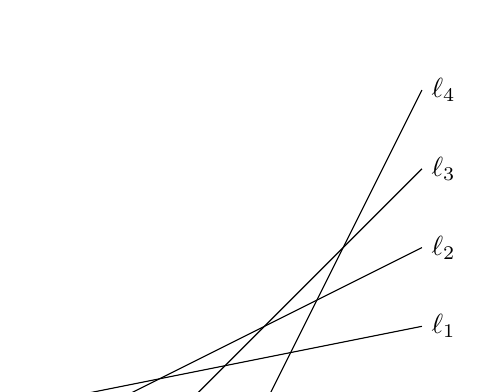
\begin{tikzpicture}[x=1cm,y=1cm]
    
    % \draw[->] (-1,0) -- (4,0)   node[right] {$x$};
    % \draw[->] (0,-1) -- (0,4)   node[above] {$y$};

    \draw (-1,0) -- (4,1) node[anchor=west]{$\ell_1$};
    \draw (0,0) -- (4,2) node[anchor=west]{$\ell_2$};
    \draw (1,0) -- (4,3) node[anchor=west]{$\ell_3$};
    \draw (2,0) -- (4,4) node[anchor=west]{$\ell_4$};
    \end{tikzpicture}
\end{center}

We say that a region is ``on the right'' if it has \( x \)-coordinate unbounded above (note that if we only have one wall, then both regions are on the right). We claim inductively that, after placing \( n \) lines, there are \( n + 1 \) connected components in the resulting labyrinth, each of which contains exactly one region on the right. This is certainly true after placing \( 0 \) lines, as then there is only one region (and hence one connected component) and it is on the right. When placing the \( n \)th line, it then cuts every one of the \( n - 1 \) previously placed lines, and since it is to the right of all intersection points, the regions it cuts are exactly the \( n \) regions on the right.

\begin{center}
    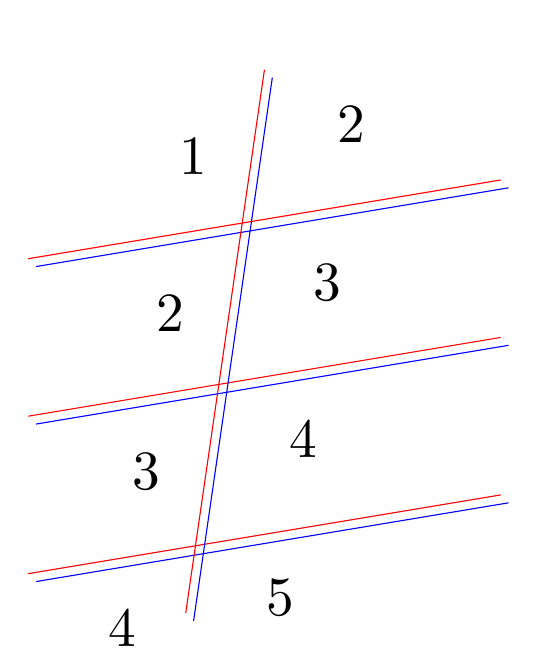
\begin{tikzpicture}[scale=2, every node/.style={transform shape}]
        \foreach \i in {1,2,3} {
            \draw[blue] (-1,\i) -- (2,\i+0.5);
            \draw[red,shift={(-0.05,0.05)}] (-1,\i) -- (2,\i+0.5);
        }

        \draw[blue] (0.5,4.2) -- (0, 0.75);
        \draw[red,shift={(-0.05,0.05)}] (0.5,4.2) -- (0, 0.75);

        \node at (0,3.7) {1};
        \node at (1,3.9) {2};

        \node[shift={(-0.15,-1)}] at (0,3.7) {2};
        \node[shift={(-0.15,-1)}] at (1,3.9) {3};

        \node[shift={(-0.3,-2)}] at (0,3.7) {3};
        \node[shift={(-0.3,-2)}] at (1,3.9) {4};

        \node[shift={(-0.45,-3)}] at (0,3.7){4};
        \node[shift={(-0.45,-3)}] at (1,3.9){5};
        
    \end{tikzpicture}
\end{center}

The addition of this line leaves all previous connected components with exactly one region on the right, and creates a new connected component containing exactly one region, and that region is also on the right. As a result, by induction, this particular labyrinth will have \( n + 1 \) connected components. Having built this labyrinth, Merlin then moves the walls one-by-one (by a sequence of continuous translations and rotations of lines) into the proper position of the given labyrinth, in such a way that no two lines ever become parallel.

The only time the configuration is changed is when one wall is moved through an intersection point of two others:

\begin{figure}[h]
    \centering
    \captionsetup{labelformat=empty}
    \begin{subfigure}[b]{0.45\textwidth}
        \centering
        \captionsetup{labelformat=empty}
        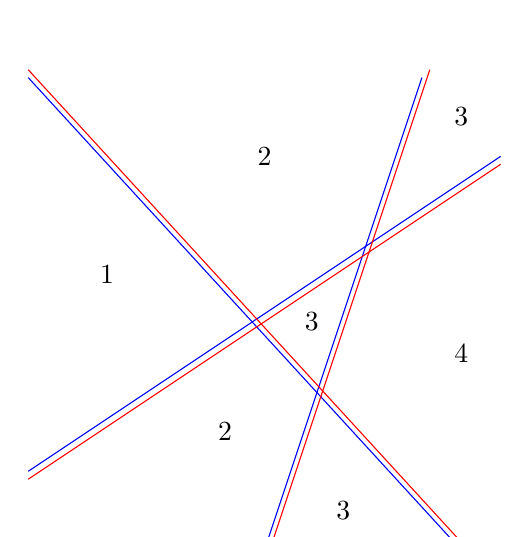
\begin{tikzpicture}
            \draw[blue] (2, 8) -- (7.5, 2);
            \draw[blue] (2, 3) -- (8, 7);
            \draw[blue] (7, 8) -- (5, 2);

            \draw[red, shift={(0,0.1)}] (2, 8) -- (7.5, 2);
            \draw[red, shift={(0,-0.1)}] (2, 3) -- (8, 7);
            \draw[red, shift={(0.1,0.1)}] (7, 8) -- (5, 2);

            \node at (3, 5.5){1} ;
            \node at (5, 7){2};
            \node at (4.5, 3.5){2} ;
            \node at (5.6, 4.9){3} ;
            \node at (7.5, 7.5){3} ;
            \node at (6, 2.5){3} ;
            \node at (7.5, 4.5){4} ;
    \end{tikzpicture}
    \end{subfigure}
    \hfill
    \begin{subfigure}[b]{0.45\textwidth}
        \centering
        \captionsetup{labelformat=empty}
        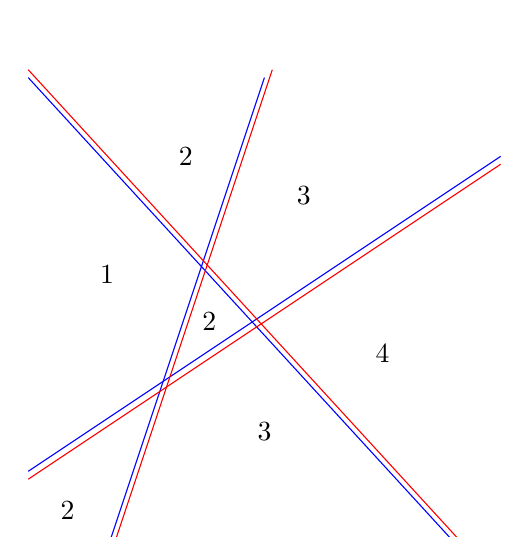
\begin{tikzpicture}
            \draw[blue] (2, 8) -- (7.5, 2);
            \draw[blue] (2, 3) -- (8, 7);
            \draw[blue,shift={(-2,0)}] (7, 8) -- (5, 2);

            \draw[red, shift={(0,0.1)}] (2, 8) -- (7.5, 2);
            \draw[red, shift={(0,-0.1)}] (2, 3) -- (8, 7);
            \draw[red, shift={(-1.9,0.1)}] (7, 8) -- (5, 2);

            \node at (3, 5.5){1} ;
            \node[shift={(-1,0)}] at (5, 7){2};
            \node[shift={(-2,-1)}] at (4.5, 3.5){2} ;
            \node[shift={(-1.3,0)}] at (5.6, 4.9){2} ;
            \node[shift={(-2,-1)}] at (7.5, 7.5){3} ;
            \node at (5, 3.5){3} ;
            \node at (6.5, 4.5){4} ;
        \end{tikzpicture}
    \end{subfigure}
\end{figure}

Note that all moves really do switch between two configurations like this: all sets of three lines have this colour configuration initially, and the rules on rotations mean they are preserved (in particular, we cannot create three lines creating a triangle with three red edges inwards, or three blue edges inwards). However, as can be seen, such a move preserves the number of connected components, so in the painting this provides for Arthur’s actual labyrinth, Morgana can still only place at most \( n + 1 \) knights.
\section{IMO 2019 SL - Problem C5}-
\section{IMO 2019 SL - Problem C8}
\begin{problem}[IMO 2019 SL - Problem C8]
Alice has a map of Wonderland, a country consisting of $n \ge 2$ towns. For every pair of towns, there is a narrow road going from one town to the other. One day, all the roads are declared to be “one way” only. Alice has no information on the direction of the roads, but the King of Hearts has offered to help her. She is allowed to ask him a number of questions. For each question in turn, Alice chooses a pair of towns and the King of Hearts tells her the direction of the road connecting those two towns.

Alice wants to know whether there is at least one town in Wonderland with at most one outgoing road. Prove that she can always find out by asking at most $4n$ questions.
\end{problem}

\subsection*{Solution.}

We will show Alice needs to ask at most $4n - 7$ questions. Her strategy has the following phases. In what follows, $S$ is the set of towns that Alice, so far, does not know to have more than one outgoing road (so initially $|S| = n$).

\subsubsection*{Phase 1}
Alice chooses any two towns, say $A$ and $B$. Without loss of generality, suppose that the King of Hearts’ answer is that the road goes from $A$ to $B$.

At the end of this phase, Alice has asked 1 question.

\subsubsection*{Phase 2}
During this phase there is a single (variable) town $T$ that is known to have at least one incoming road but not yet known to have any outgoing roads. Initially, $T$ is $B$. Alice does the following $n - 2$ times: she picks a town $X$ she has not asked about before, and asks the direction of the road between $T$ and $X$. If it is from $X$ to $T$, $T$ is unchanged; if it is from $T$ to $X$, $X$ becomes the new choice of town $T$, as the previous $T$ is now known to have an outgoing road.

At the end of this phase, Alice has asked a total of $n - 1$ questions. The final town $T$ is not yet known to have any outgoing roads, while every other town has exactly one outgoing road known. The undirected graph of roads whose directions are known is a tree.

\subsubsection*{Phase 3}
During this phase, Alice asks about the directions of all roads between $T$ and another town she has not previously asked about, stopping if she finds two outgoing roads from $T$. This phase involves at most $n - 2$ questions. If she does not find two outgoing roads from $T$, she has answered her original question with at most $2n - 3 \leq 4n - 7$ questions, so in what follows we suppose that she does find two outgoing roads, asking a total of $k$ questions in this phase, where $2 \leq k \leq n - 2$ (and thus $n \geq 4$ for what follows).

For every question where the road goes towards $T$, the town at the other end is removed from $S$ (as it already had one outgoing road known), while the last question resulted in $T$ being removed from $S$. So at the end of this phase, $|S| = n - k + 1$, while a total of $n + k - 1$ questions have been asked. Furthermore, the undirected graph of roads within $S$ whose directions are known contains no cycles. Every town in $S$ has exactly one outgoing road known.

\subsubsection*{Phase 4}
During this phase, Alice repeatedly picks any pair of towns in $S$ for which she does not know the direction of the road between them. Because every town in $S$ has exactly one outgoing road known, this always results in the removal of one of those two towns from $S$. Because there are no cycles in the graph of roads of known direction within $S$, this can continue until there are at most 2 towns left in $S$.

If it ends with $t$ towns left, $n - k + 1 - t$ questions were asked in this phase, so a total of $2n - t$ questions have been asked.

\subsubsection*{Phase 5}
During this phase, Alice asks about all the roads from the remaining towns in $S$ that she has not previously asked about. She has definitely already asked about any road between those towns (if $t = 2$). She must also have asked in one of the first two phases about at least one other road involving one of those towns. So she asks at most $t(n - t) - 1$ questions in this phase.

At the end of this phase, Alice knows whether any town has at most one outgoing road.

If $t = 1$, at most $3n - 3 \leq 4n - 7$ questions were needed in total, while if $t = 2$, at most $4n - 7$ questions were needed in total.
\section{IMO 2019 SL - Problem C9}-

\chapter{Competitive programming problems}

\chapter{Graph problems}
% Un sujet ENS
\section{Combinatorics problems}-

\bibliographystyle{plain}
\bibliography{bib/articles,bib/books,bib/misc}

\end{document}